% !TeX document-id = {ecd2ddc3-3e72-4f39-ab15-a36e01d4af13}
%!TEX TS-program = /usr/texbin/pdflatex
%!GEDIT texbin = /usr/local/texlive/current/bin/x86_64-linux/pdflatex
%
%	''Becker-Vorlage'' style LaTeX template

% 	This template is  MIT licensed, authors:
%   Jan Betzing <jan.betzing@ercis.uni-muenster.de> *corresponding author
%	Dominik Lekse <dominik@lekse.de>
%
% 	Basic file to demonstrate the usage of this LaTeX template.
% 	You can build your own paper/thesis on top of this file.
% 	Simply adjust the document class and all metadata and start working.
%
\documentclass[
	language=english, % set to english or german
	type=seminar % set to bachelor, master or seminar
]{isthesis}

% Graphics rendering using TikZ
% See: https://en.wikibooks.org/wiki/LaTeX/PGF/TikZ
\usepackage{tikz}
% Include required TikZ libraries here, some exemplary libraries are pre-included
\usetikzlibrary{calc}
\usetikzlibrary{matrix}
\usetikzlibrary{positioning}
\usetikzlibrary{shapes.geometric}

% Import acronyms
% \newacronym[longplural={<long plural>}, shortplural={<short plural>}]{<label>}{<short>}{<long>}
% 	label = is the unique identifier and sort key for the acronym, can be the same as <short>
%	short = is the abbreviation or acronym
%	short plural (optional) = is the plural of the abbreviation or acronym
%	long = is the long form of the acronym, this will appear in the list of abbreviations
%	long plural (optional) = is the long plural form of the abbreviation or acronym

\newacronym[shortplural={KMUen}, longplural={Kleine und Mittlere Unternehmen}]{kmu}{KMU}{Kleines und Mittleres Unternehmen}
\newacronym{CD}{CD}{Corporate Design}
\newacronym{SQL}{SQL}{Structured Query Language}
\newacronym{ERCIS}{ERCIS}{European Research Center for Information Systems}
\newacronym{WWU}{WWU}{Westf\"alische Wilhelms-Universit\"at}
\newacronym{BPM}{BPM}{Business Process Management}
\newacronym{npm}{NPM}{Node Package Manager}

% Import symbols
% Syntax: <Symbol> <Label> <Name>
% The symbols are sorted by their labels
\addsymboltolist{$\Pi$}{Pi}{Projection}
\addsymboltolist{$\Join$}{Join}{Natural Join}
\addsymboltolist{$\sigma$}{Selection}{Selection}


% Document meta information
\isthesis{
    title={An Investigation in the Springleaf Kaggle Challenge},
    author={Marcus Cramer, Markus Heuchert},
    author-email={ \{m\_heuc03, m\_cram02\}@uni-muenster.de},
    author-phone={+49 251 8338100}, % Use international numbers format
    author-matriculation={385413},
    author-address={Schlossplatz 2},
    author-zip={48149},
    author-city={M\"{u}nster},
    principal-supervisor={Prof. Dr. Heike Trautmann}, % This has to be a professor
    tutor-supervisor={Matthias Carnein, M.Sc.}, % This is your main supervisor, i.e., a post doc or PhD student
    tutor-supervisor={Pascal Kerschke, M.Sc.}, % If required, define an additional supervisor resp. tutor here
    group={Chair for Information Systems and Statistics},
    group-institute={Westphalian Wilhelms-University, M\"unster},
    %associate-group={}, % When the thesis is done in cooperation with another chair, add it here
    %associate-group-institute={}, % add cooperating institute or university here
    seminar={Applied Machine Learning}, % The title of your seminar
    submission-date={2017-01-10}, % The date you handed in your document
    %primary-logo={}, % Uses the WWU logo by default
    %primary-logo-height={}, % Uses 16mm as default height
    %secondary-logo={}, % Logo of the secondary institution (cooperating chair/university), USES Faculty logo by default
    %secondary-logo-height={} % Uses 16mm as default height
}
\begin{document}
    % Title page
    \maketitle

	% Quote
    % You can put an optional quote page in front of your content
   %\quotepage[author={Arthur C. Clarke}]{
   	%        Any sufficiently advanced technology is indistinguishable from magic.
   %}

    % Table of contents
    \tableofcontents

    % List of figures (if you have figures)
    \listoffigures

    % List of tables (if you have tables)
    \listoftables
    
    % List of listings (if you have listings)
	\lstlistoflistings

    % List of abbreviations (if you use acronyms)
    \listofabbreviations

    % List of symbols (if you use symbols)
    \listofsymbols

	% Abstract
	%
	% Comment out this part, if you don't require an abstract
	\begin{abstract}
		This paper documents the investigation in the springleaf marketing response challenge held on kaggle from August to October 2015. Its goal was to predict whether to send a direct mail piece to a customer through mining a large data set consisting of 1933 features and 145232 rows in the training set. The features hold anonymized customer information and there is a binary outcome, which is to predict. Since the challenge is over, we are able to compare our performance with the winners of the competition. OUR SOLUTION USES XGBOOST AND ACHIEVES AN AREA UNDER CURVE SCORE OF.....
	\end{abstract}

    % Content
    \begin{content}
		%!TEX root = ./00_thesis.tex
%!GEDIT texmaster = ./00_thesis.tex
\chapter{Introduction}

Springleaf offers their customers loans and direct mail is one important way to connect with customers whom may be in need of a loan. The identification of good candidates for their services is essential for the successful execution of their marketing strategy. The data set at hand consists of nearly 2000 features that hold anonymized customer information. The goal is to predict their response to an offering, which is the binary target variable. A training and test set of equal size is provided, each with nearly 150000 records. 

This documentation reasons our approach to create a powerful, yet performant predictor. 


\chapter{Data Set}

\chapter{Predicting Marketing Response}

\chapter{Discussion}

\chapter{TEMPLATE INTRODUCTION}
This \LaTeX \- template has been developed as an alternative to the well-known Microsoft Word \enquote{Becker-Vorlage}. \path{00_thesis.tex} is the master file.

It is build by  Jan Betzing and Dominik Lekse and draws from the DBIS template by Till Haselmann and Florian Stahl, as well as from the IS template by Stephan Dlugosz.

This document is work-in-progress and provides instructions on how to use the template. It does not give advices on scientific writing.

Please feel free to contribute to this template. Members of the WWU M\"{u}nster can request access to the template by contacting the author at \href{mailto:jan.betzing@ercis.uni-muenster.de}{jan.betzing@ercis.uni-muenster.de}. Afterwards you will be able to clone the template from \path{https://wiwi-gitlab.uni-muenster.de/lsis/isthesis.git}, and create push-requests with their new features.

\paragraph{TODO}
\begin{itemize}
	\item Configuration switch for having \textbackslash chapter\{\} begin on a new page
	\item Replace \texttt{kvoptions} with \texttt{pgfkeys}
\end{itemize}
\chapter{TEMPLATE ELEMENTS}
This chapter gives examples on what you can do with this template. It's just a brief overview. Please consult the common sources on how to write sicentific documents and documents with \LaTeX.

\section{Structure}
This template provides three structural levels that appear in the table of contents, \viz, \texttt{\textbackslash chapter}, \texttt{\textbackslash section}, and \texttt{\textbackslash subsection}. Chapters will always start on a new page. Additionally, you can use \texttt{\textbackslash subsubsection} and \texttt{\textbackslash paragraph} as non-hierarchical means to structure your thesis.


\subsection{Lists}
You can use the default \LaTeX \- functions for writing lists, \viz, \texttt{\textbackslash enumerate} for numbered lists and \texttt{\textbackslash itemize} for bullet point lists. Again, the \texttt{\textbackslash subsubsection} and \texttt{\textbackslash paragraph} can be used as structural elements, \eg, when listing definitions of terms.

\subsection{Footnotes}
Footnotes are contiguously numbered throughout the whole document. Use the \texttt{\textbackslash footnote\{text\}} command.  They appear on the page their reference is on \footnote{This is an exemplary footnote.}. Footnotes have to be placed without whitespace behind the word and within the sentence boundaries, \ie, before the period.

\subsection{ToDo-Notes}
You can use ToDo notes using the \texttt{\textbackslash todo\{text\}}  command. Please make sure to remove any ToDo notes before handing in your thesis! \todo[inline]{ToDo: Remove me before publishing}

\section{Formatting Text}
\LaTeX \- provides \texttt{\textbackslash textit\{text\}} for \textit{italics}, \texttt{\textbackslash textbf\{text\}} for \textbf{bold face}, \texttt{\textbackslash texttt\{text\}} for \texttt{typewriter}, \texttt{\textbackslash textsc\{text\}} for \textsc{small caps}, \texttt{\textbackslash underline\{text\}} for \underline{underline}. Additionally, the template provides  \texttt{\textbackslash texthl\{text\}} for \texthl{highlighted text}. Please remove any highlighted text before handing in your thesis!

Please use the \texttt{\textbackslash enquote\{text\}} command for \enquote{direct quotes}.

\subsection{Colors}
This template comes with the colors defined in the \glspl{CD} of the \acrshort{ERCIS} and \acrshort{WWU}. \Tab \ref{tab:colors} lists the color names. You can apply them to text by using the  \\ \texttt{\textbackslash textcolor\{color name\}\{text\}} command.
	
\begin{table}[caption={Colors defined by the template}, label=tab:colors]
	\centering
		\begin{tabular}{@{}ll@{}}
			\toprule
			{\bf Color Name} & {\bf Result} \\ \midrule
			ercis-black      & \textcolor{ercis-black}{Exemplary Text and 0123456789}  \\
			ercis-grey      & \textcolor{ercis-grey}{Exemplary Text and 0123456789}  \\
			ercis-red      & \textcolor{ercis-red}{Exemplary Text and 0123456789}  \\
			ercis-lightred      & \textcolor{ercis-lightred}{Exemplary Text and 0123456789}  \\
			ercis-blue      & \textcolor{ercis-blue}{Exemplary Text and 0123456789}  \\
			ercis-darkblue      & \textcolor{ercis-darkblue}{Exemplary Text and 0123456789}  \\
			ercis-cyan    & \textcolor{ercis-cyan}{Exemplary Text and 0123456789}  \\
			ercis-orange      & \textcolor{ercis-orange}{Exemplary Text and 0123456789}  \\
			ercis-green      & \textcolor{ercis-green}{Exemplary Text and 0123456789}  \\ \midrule
			wwu-black      & \textcolor{wwu-black}{Exemplary Text and 0123456789}  \\
			wwu-green      & \textcolor{wwu-green}{Exemplary Text and 0123456789}  \\
			wwu-lightgreen      & \textcolor{wwu-lightgreen}{Exemplary Text and 0123456789}  \\
			wwu-blue     & \textcolor{wwu-blue}{Exemplary Text and 0123456789}  \\
			wwu-lightblue      & \textcolor{wwu-lightblue}{Exemplary Text and 0123456789}  \\ \bottomrule
		\end{tabular}
\end{table}


\section{Figures}

The \texttt{figure} environment is wrapped around images. These images should either be included as PDF-file via \texttt{\textbackslash includegraphics}, or created via \textit{TikZ/PGF}. For included images, make sure to use high-resolution images, preferably vector images.

Figures float, \ie, they do not necessarily appear at exact the same position you have defined them. Make sure to set a  \textit{caption} and an optional \textit{label} as figure parameters. 

\begin{figure}[caption={Relationship of students and theses}, label={fig:img01}]
	{	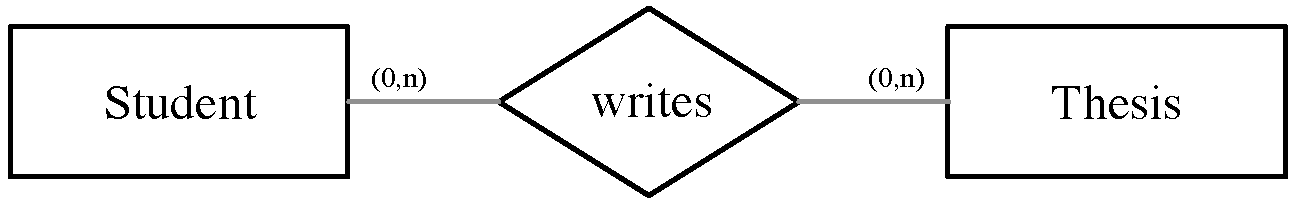
\includegraphics[width=.6\textwidth]{figures/figure01.pdf}}
\end{figure}

\subsection{Subfigures}
Sometimes it might be handy to contrast figures, \ie, by placing them next to each other. The template uses the \textit{subcaption} package to provide subfigures. The following example contains two figures, where each subfigure has its own \texttt{\textbackslash label} and \texttt{\textbackslash caption}. Additionally, the whole figure has its own \textit{caption} and \textit{label}. That means, you can reference subfigures  \fig \ref{fig:subfig1} and \fig  \ref{fig:subfig}. Only the whole figure will be listed in the table of figures.

Subfigures are not limited to images, but may also include listings or tables. \Fig \ref{fig:subfig} shows a sample database query expressed in \ac{SQL} (\fig \ref{fig:subfig1}) and as query plan in relational algebra  (\fig \ref{fig:subfig2}).
 
\begin{figure}[caption={Exemplary use of subfigures}, label={fig:subfig}]
	
	\begin{subfigure}[b]{.45\textwidth}
		
		\begin{lstlisting}[nolol, language=SQL]
		SELECT b, d FROM 
			EXAMPLE.RELATION1 r,
			EXAMPLE.RELATION2 s,
		WHERE 
			r.a = 'c'
		AND 
			s.e = 2
		AND 
			r.c = s.c; 
		\end{lstlisting}
		\caption{\gls{SQL} select statement}\label{fig:subfig1}
	\end{subfigure}
	\begin{subfigure}[b]{.53\textwidth}
		\centering	
		\begin{tikzpicture}[node distance = 2cm, auto,
		database/.style={
			cylinder,
			cylinder uses custom fill,
			cylinder body fill=gray!30,
			cylinder end fill=gray!20,
			shape border rotate=90,
			aspect=0.25,
			draw
		}]
		\node [] (queue) {$\Pi_{b, d}$};
		\node [below of=queue] (join) {$\Join_{r.c = s.c}$};
		
		\node [below left of=join,xshift=-1cm] (l1) {$\sigma_{r.a = 'c'}$};
		\node [database, below of=l1] (l2) {\texttt{r}};
		
		\node [below right of=join,xshift=1cm] (r1) {$\sigma_{s.e = 2}$};
		\node [database,below of=r1] (r2) {\texttt{s}};
		
		\draw [<-] (queue) -- (join);
		\draw [<-] (join) -- (r1);
		\draw [<-] (r1) -- (r2);
		\draw [<-] (join) -- (l1);
		\draw [<-] (l1) -- (l2);
		\end{tikzpicture}
		\caption{Sample evaluation plan}\label{fig:subfig2}
	\end{subfigure}
\end{figure}
\section{Listings}
You can use listings to typeset source code. This template uses the \textit{listings} package. Wrap code inside the \texttt{lstlisting} environment and set the \textit{language} (e.g., Java, SQL), \textit{caption}, and optional \textit{label} parameters. If the source code highlighting highlights the wrong keywords or misses keywords, use the \textit{deletekeywords} \resp \textit{morekeywords} parameters. Consult the package documentation for further information.

\begin{lstlisting}[float=htp, caption={Euclid's GCD algorithm implemented in Java}, label={lst:euclid}, language=Java, deletekeywords={}, morekeywords={}]
public class Euclid {

	public static int gcd(int p, int q) {
		if (q == 0) return p;
		else return gcd(q, p % q);
	}

}
\end{lstlisting}

\section{Algorithms}
Some users might require specifying algorithms. This template uses the \textit{algorithm}, \textit{algorithmicx}, and \textit{algopseudocode} packages. Consult the respective manuals for further information. Algorithms do not appear in a table at the beginning of the document, \ie, there is no list of algorithms.

\begin{algorithm}[htb]
	\begin{algorithmic}
		\Require nonnegative integer $a$, nonnegative integer $b$
		\Function{Euclid}{$a, b$}
		\If {$b = 0$} \Comment{comment}
		\State{return $a$;}
		\Else 
		\State {return \textsc{Euclid}$(b, a\mod b)$;}
		\EndIf
		\EndFunction
	\end{algorithmic}
	\caption{Euclid's GCD algorithm in pseudocode}
	\label{alg:garbage}
\end{algorithm}

\section{Acronyms and Abbreviations}
This template provides comprehensive support for acronyms and abbreviations. The template uses the \textit{glossaries} package. 
Please do only define abbreviations and symbols that are uncommon. That means, common abbreviations such as \enquote{\eg} or \enquote{\ie} should not be listed. Abbreviations and symbols are sorted automatically by their label. 

\subsection{Common Abbreviations}
Please note that each full stop in a common abbreviation should be followed by a non-breaking space. This template comes with a variety of macros for common abbreviations, that can be used throughout your theses. The macros differ for English and German theses. Please see the tables below.

\begin{table}[caption={Common abbreviation macros for English theses}, label=tab:macros1]
	\centering
	\begin{tabular}{@{}ll@{}}
		\toprule
		{\bf Command} & {\bf Result} \\ \midrule
			\textbackslash apprx      & \apprx \\
			\textbackslash as      & \as \\
			\textbackslash cf      & \cf \\
			\textbackslash eg      & \eg \\
			\textbackslash Eg      & \Eg \\
			\textbackslash esp      & \esp \\
			\textbackslash etal      & \etal \\
			\textbackslash fig      & \fig \\
			\textbackslash Fig     & \Fig \\
			\textbackslash ie      & \ie \\
			\textbackslash Ie      & \Ie \\
			\textbackslash iid      & \iid \\
			\textbackslash p\{4711\}      & \p{4711} \\
			\textbackslash pf\{4711\}      & \pf{4711} \\
			\textbackslash pp\{11$--$47\}      & \pp{11--47} \\
			\textbackslash resp      & \resp \\
			\textbackslash sect     & \sect \\
			\textbackslash tab      & \tab \\
			\textbackslash Tab      & \Tab \\
			\textbackslash viz      & \viz \\
			\textbackslash wrt      & \wrt \\ \bottomrule
	\end{tabular}
\end{table}

\begin{table}[caption={Common abbreviation macros for German theses}, label=tab:macros2]
	\begin{subfigure}[t]{.45\textwidth}
	\centering
	\begin{tabular}{@{}ll@{}}
		\toprule
		{\bf Command} & {\bf Result} \\ \midrule
\textbackslash aaO & \mbox{a.\,a\,O}\xdot \\
\textbackslash Abb & \mbox{Abb.~} \\
\textbackslash bspw & \mbox{bspw}\xdot \\
\textbackslash bzgl & \mbox{bzgl}\xdot \\
\textbackslash bzw & \mbox{bzw}\xdot \\
\textbackslash ca & \mbox{ca}\xdot \\
\textbackslash dgl & \mbox{dgl}\xdot \\
\textbackslash dsgl & \mbox{dsgl}\xdot \\
\textbackslash dh & \mbox{d.\,h}\xdot \\
\textbackslash etc & \mbox{etc}\xdot \\
\textbackslash eV & \mbox{e.\,V}\xdot \\
\textbackslash evtl & \mbox{evtl}\xdot \\
\textbackslash fs & \mbox{f.\,s}\xdot \\
\textbackslash gdw & \mbox{g.\,d.\,w}\xdot \\
\textbackslash ggf & \mbox{ggf}\xdot \\
\textbackslash hc & \mbox{h.\,c}\xdot \\
\textbackslash iAllg & \mbox{i.\,Allg}\xdot \\
\textbackslash iBa & \mbox{i.\,B.\,a}\xdot \\
\textbackslash idR & \mbox{i.\,d.\,R}\xdot \\
\textbackslash ieS & \mbox{i.\,e.\,S}\xdot \\
\textbackslash inkl & \mbox{inkl}\xdot \\
\textbackslash insb & \mbox{insbes}\xdot \\
\textbackslash Prof & \mbox{Prof}\xdot \\
\textbackslash Dr & \mbox{Dr}\xdot \\
\textbackslash PD & \mbox{PD}\xdot \\
\textbackslash Ing & \mbox{Ing}\xdot \\
\textbackslash iV & \mbox{i.\,V}\xdot \\
\textbackslash iW & \mbox{i.\,W}\xdot \\
\textbackslash iwS & \mbox{i.\,w.\,S}\xdot \\
\textbackslash Nr\{123\} & \mbox{Nr.~123} \\
\textbackslash nW & \mbox{n.\,W}\xdot \\
\textbackslash oa & \mbox{o.\,a}\xdot \\
\textbackslash oAe & \mbox{o.\,\"{A}}\xdot \\
			\textbackslash oae & \mbox{o.\,\"{a}}\xdot \\\bottomrule
\end{tabular}
\end{subfigure}
	\begin{subfigure}[position=t]{.45\textwidth}
		\centering
		\begin{tabular}{@{}ll@{}}
			\toprule
			{\bf Command} & {\bf Result} \\ \midrule

			\textbackslash oE & \mbox{o.\,E}\xdot \\
			\textbackslash oEdA & \mbox{o.\,E.\,d.\,A}\xdot \\
			\textbackslash OEdA & \mbox{O.\,E.\,d.\,A}\xdot \\ 
			\textbackslash oV & \mbox{o.\,V}\xdot \\
			\textbackslash OV & \mbox{O.\,V}\xdot \\
			\textbackslash resp & \mbox{resp}\xdot \\
			\textbackslash S\{123\} & \mbox{S.~123} \\
			\textbackslash Sf\{123\} & \mbox{S.~123~f}\xdot \\
			\textbackslash Sff\{123\} & \mbox{S.~123~ff}\xdot \\
			\textbackslash siehe & \mbox{s.\,o}\xdot \\
			\textbackslash sog & \mbox{sog}\xdot \\
			\textbackslash sS\{123\}  & \mbox{s.\,S.~123}\\
			\textbackslash sSf\{123\} &\mbox{s.\,S.~123~f}\xdot \\
			\textbackslash sSff\{123\}& \mbox{s.\,S.~123~ff}\xdot \\
			\textbackslash stu & \mbox{st.\,u}\xdot \\
			\textbackslash su & \mbox{s.\,u}\xdot \\
			\textbackslash Tab & \mbox{Tab.~} \\
			\textbackslash tw & \mbox{t.\,w}\xdot \\
			\textbackslash ua & \mbox{u.\,a}\xdot \\
			\textbackslash etal & \mbox{et\ al}\xdot \\
			\textbackslash uae & \mbox{u.\,\"{a}}\xdot \\
			\textbackslash uAe & \mbox{u.\,\"{A}}\xdot \\
			\textbackslash uiv & \mbox{u.\,i.\,v}\xdot \\
			\textbackslash usw & \mbox{usw}\xdot \\
			\textbackslash uU & \mbox{u.\,U}\xdot \\
			\textbackslash va & \mbox{v.\,a}\xdot \\
			\textbackslash vgl & \mbox{vgl.~} \\
			\textbackslash Vgl & \mbox{Vgl.~} \\
			\textbackslash vs & \mbox{v.\,s}\xdot \\
			\textbackslash zB & \mbox{z.\,B}\xdot \\
			\textbackslash zT & \mbox{z.\,T}\xdot \\
			\textbackslash zz & \mbox{zz}\xdot \\
			\textbackslash zzgl & \mbox{zzgl}\xdot \\
 & \\ \bottomrule
	\end{tabular}
	\end{subfigure}
\end{table}

\subsection{Custom Abbreviations}
Custom abbreviations are defined in the \path{acronyms.tex} file, using the \\
\texttt{\textbackslash newacronym[longplural=\{<long plural>\}, shortplural=\{<short plural>\}]\\ \{<label>\}\{<short>\}\{<long>\}} command. The \textit{longplural} and \textit{shortplural} parameters are optional. The abbreviations are sorted by their labels. The label is furthermore used to reference the abbreviations in your text. You can do so using commands listed in \tab \ref{tab:glossaries}. In most cases, you just use \textbackslash gls\{<label>\}. On the first occurrence, the full version is displayed, \eg, \acrfull{ERCIS}. Afterwards, the short version will be displayed, \eg, \acrshort{ERCIS}.

You pluralize your abbreviation by adding a \texttt{pl} to the \resp command. This will add a small s to the abbreviation, \eg, \acrshortpl{CD}. \Tab \ref{tab:glossaries} shows custom short and long plural versions of the abbreviation \acrshort{kmu}. You might need this \esp for more complex German abbreviations that do not have a \enquote{s} plural form.

\begin{table}[caption={Commands for printing abbreviations}, label=tab:glossaries]
	\centering
	\begin{tabular}{@{}ll@{}}
		\toprule
		{\bf Command} & {\bf Result} \\ \midrule
		\textbackslash gls\{<label>\}     & \textbackslash acrfull on first occurence, \textbackslash acrshort otherwise \\
		\textbackslash glspl\{<label>\}       &  \textbackslash acrfullpl on first occurence, \textbackslash acrshortpl otherwise \\
		\textbackslash acrshort\{<label>\}       & \acrshort{kmu} \\
		\textbackslash acrshortpl\{<label>\}       & \acrshortpl{kmu} \\
		\textbackslash acrlong\{<label>\}       & \acrlong{kmu} \\
		\textbackslash acrlongpl\{<label>\}      & \acrlongpl{kmu} \\
		\textbackslash acrfull\{<label>\}      & \acrfull{kmu} \\
		\textbackslash  acrfullpl\{<label>\}     & \acrfullpl{kmu} \\ \bottomrule
	\end{tabular}
\end{table}

Only referenced abbreviations will be added to the list of abbreviations.

\subsection{Symbols}
If required, you can define symbols in the \path{symbols.tex} file, using the \\ \texttt{\textbackslash addsymboltolist\{<symbol>\}\{<label>\}\{<name>\}} command. The symbols are sorted by their labels. Please note, regardless of using the symbols in the text, all symbols defined in the symbols file will be output to the list of symbols.

\section{Citations and Bibliography}
This template uses {BibTeX} for bibliographies. It comes with the MISQ style that takes care of proper formating and sorting of your references. Of course, you have to maintain a clean \path{.bib} file that caters all necessary attributes. References will appear in the alphabetical order of the surname of the first author. In case of several works by the same author, they are sorted by year.

Citing in the text is done with the \textbackslash citep[<before>][<after>]\{<citekey>\} command. Citations without parenthesis are done with \textbackslash cite\{<citekey>\}. You can reference authors with \textbackslash citeauthor\{<citekey>\}. However, we suggest typesetting authors in \textsc{Small Caps}, \eg, \textsc{\citeauthor{Hammer2015}} is one father of \ac{BPM}.

\paragraph{Exemplary citations}

\begin{itemize}
	\item \gls{BPM} is an integral management paradigm for building and running effective and efficient organizations  \citep{Hammer2015, VomBrocke2014a}.
	\item A holistic approach to \ac{BPM} goes beyond process modeling and workflow management systems \citep[\p{530}]{VomBrocke2014a}.
	\item See \cite{VomBrocke2014a} for a comprehensive review on \ac{BPM} best practices.
	\item \textsc{\citeauthor{Hammer2015}} lists organizational capabilities for \ac{BPM} \citep[\cf][\pf{9}]{Hammer2015}, while \textsc{vom Brocke} \etal give principles of good \ac{BPM} \citep[\cf][\pp{530--546}]{VomBrocke2014a}.
	\item Two authors are automatically divided by an \enquote{and} in English or an \enquote{und} in German, \eg, \citep{Becker2011}.
	\item \enquote{\ac{BPM} can provide a solid set of capabilities essential to master contemporary and future challenges} \citep[\p{534}]{VomBrocke2014a}.
\end{itemize}

\subsection{Misc}
The name and matriculation number of the student will automatically be displayed on the header of every page when the thesis type \textit{seminar} is selected.

\chapter{TEMPLATE COMPILING}
In order to generate a PDF-file from your \TeX-file you have to run the following commands. We assume you have a master file \path{00_thesis.tex} that you want to typeset.

\begin{lstlisting}[float=htp, caption={Commands to compile this document}, label={lst:compiling}, language=bash, morekeywords={pdflatex, bibtex, makeglossaries}]
pdflatex 00_thesis
pdflatex 00_thesis
makeglossaries 00_thesis
bibtex 00_thesis
pdflatex 00_thesis
pdflatex 00_thesis
\end{lstlisting}

Alternatively, you can use your favorite task runner. This thesis comes with a \textit{Grunt} file to kick-start your \LaTeX writing.

When running, Grunt will monitor your thesis and on file changes, the PDF-file is automatically rebuild using the commands from listing \ref{lst:compiling}.
 
Please make sure to have node.js and the \gls{npm} installed. Now you can open a command prompt at the document root and run the commands in listing \ref{lst:grunt}. 

\begin{lstlisting}[float=htp, caption={Installing and running Grunt}, label={lst:grunt}, language=bash]
# Install Grunt via npm (use sudo on Unix-based OS)
npm install -g grunt-cli

# Install Grunt plugins / dependencies
npm install

# Run the Grunt listener 
grunt
\end{lstlisting}
		% Add your content files here
    \end{content}

    % Appendix
     \begin{appendix}
         \section{Some Appendix Section}\label{sec:appendix01}
Appendices provide only two structural levels, \viz, \texttt{\textbackslash section}, and \texttt{\textbackslash subsection}.

The numbering of figures, listings, tables, and footnotes is not reset. Thus, it continues as usual in the appendix.

\subsection{Some Appendix Subsection}

\lipsum[10]
     \end{appendix}

    % References
    \references{library}

    % Declaration of authorship
    % \authorshipstatement[pagenumbering=false]
    \authorshipstatement[pagenumbering=true]
    % \authorshipstatement[pagenumbering=only]
    
    % Bonus: Wordcount
    % cd %FOLDER WHERE THE .tex FILES ARE IN %
    % clear
    % texcount -total -q -col -sum *.tex
    
\end{document}